\subsection{The Pythagoreans: When Math Becomes a Cult}

While the Egyptians were busy using math to keep their fields square and their temples standing, the Pythagoreans had other plans. They didn’t just use ratios — they worshipped them.

To the followers of Pythagoras (yes, the triangle guy), numbers weren’t just practical tools — they were sacred. They believed that everything in the universe could be explained through whole-number ratios: music, motion, the stars, your mood swings — you name it.

\begin{quote}
\textit{“All is number.”} – Pythagoras, probably while staring meaningfully into space.
\end{quote}

\subsubsection*{Hearing the Ratios: How Math Made the Universe Hum}

The Pythagoreans weren’t just playing with triangles — they were listening to the cosmos. One of their most mind-blowing discoveries came not from the sky, but from a stretched string.

They found that if you pluck a string and then divide its length in half, the resulting note is exactly one octave higher — a perfect \(2:1\) ratio. Divide it into a \(3:2\) proportion, and you get a fifth. A \(4:3\) gives you a fourth. These weren’t just pleasing sounds — they were mathematical truths hiding in plain hearing.

To them, this was no coincidence. It meant the universe itself was whispering in ratios. The fact that harmony — the most emotionally resonant, divine, and ineffable of experiences — could be reduced to clean numerical relationships was like discovering a hidden order beneath reality. 

If strings on a lyre could obey mathematics, why not the stars? The Pythagoreans imagined that the planets, too, moved through space like cosmic instruments — each with its own tone, each orbit tracing a chord in a silent, eternal symphony. You couldn't hear it with your ears, but with the right math, you could \textit{feel} it.

This was more than science. It was a philosophy. A theology. A revelation that the abstract world of number had slipped its chains — and was now humming through the universe.

\medskip

\begin{figure}[H]
   \centering
   \begin{tikzpicture}[scale=3.0, every node/.style={font=\scriptsize}]
   
   % Full string (length = 3.0)
   \draw[thick] (0,0) -- (3,0);
   \filldraw[black] (0,0) circle (0.5pt);
   \filldraw[black] (3,0) circle (0.5pt);
   \node[below] at (0,0) {0 (Bridge)};
   \node[below] at (3,0) {1 (Nut)};
   %\node[below=4pt] at (1.5,0) {String length};
   
   % Harmonic division points
   \draw[dashed] (1.5,0) -- (1.5,0.8); % 2:1 (octave)
   \draw[dashed] (2.0,0) -- (2.0,0.8); % 3:2 (fifth)
   \draw[dashed] (2.25,0) -- (2.25,-0.8); % 4:3 (fourth)
   
   \filldraw[red] (1.5,0) circle (0.5pt);
   \filldraw[red] (2.0,0) circle (0.5pt);
   \filldraw[red] (2.25,0) circle (0.5pt);
   
   % Fraction labels aligned with red dots
   \node[below=3pt] at (1.5,0) {\footnotesize \(\frac{1}{2}\)};
   \node[below=3pt] at (2.0,0) {\footnotesize \(\frac{2}{3}\)};
   \node[below=3pt] at (2.25,.25) {\footnotesize \(\frac{3}{4}\)};
   
   % Ratio labels
   \node[above] at (1.5,0.8) {\(2:1\)};
   \node[above] at (2.0,0.8) {\(3:2\)};
   \node[below] at (2.25,-0.8) {\(4:3\)};
   
   % Arcs showing harmonic intervals
   \draw[blue!70!black, thick, ->] (1.5,0.8) arc[start angle=90, end angle=135, radius=1.2]
       node[midway, above left] {\small Octave};
   
   \draw[green!60!black, thick, ->] (2.0,0.8) arc[start angle=90, end angle=45, radius=1.2]
       node[midway, above right] {\small Fifth};
   
   \draw[orange!80!black, thick, ->] (2.25,0) arc[start angle=270, end angle=315, radius=1.5]
       node[midway, above left] {\small Fourth};
   
   \end{tikzpicture}
   \caption{An extended string shows how dividing at precise ratios produces musical intervals. The octave (\(2:1\)), fifth (\(3:2\)), and fourth (\(4:3\)) were central to Pythagorean music theory — a harmony hiding in plain sight.}
\end{figure}
   
\medskip   
   
   


\subsubsection*{The Harmony of the Spheres: When Astronomy Got Really Into Music Theory}

And so they developed what would become known as the \textbf{harmony of the spheres}: the idea that the planets orbited in perfect circles, spaced according to divine musical ratios. They couldn't hear this cosmic music, but they were convinced it was there — a kind of silent, celestial jazz.

To describe planetary motion, they began to craft early models using circles, spheres, and proportional distances. While not physically accurate, these models introduced the concept that mathematics could describe motion and structure beyond immediate human experience — a giant leap toward mathematical astronomy.

\begin{figure}[H]
   \centering
   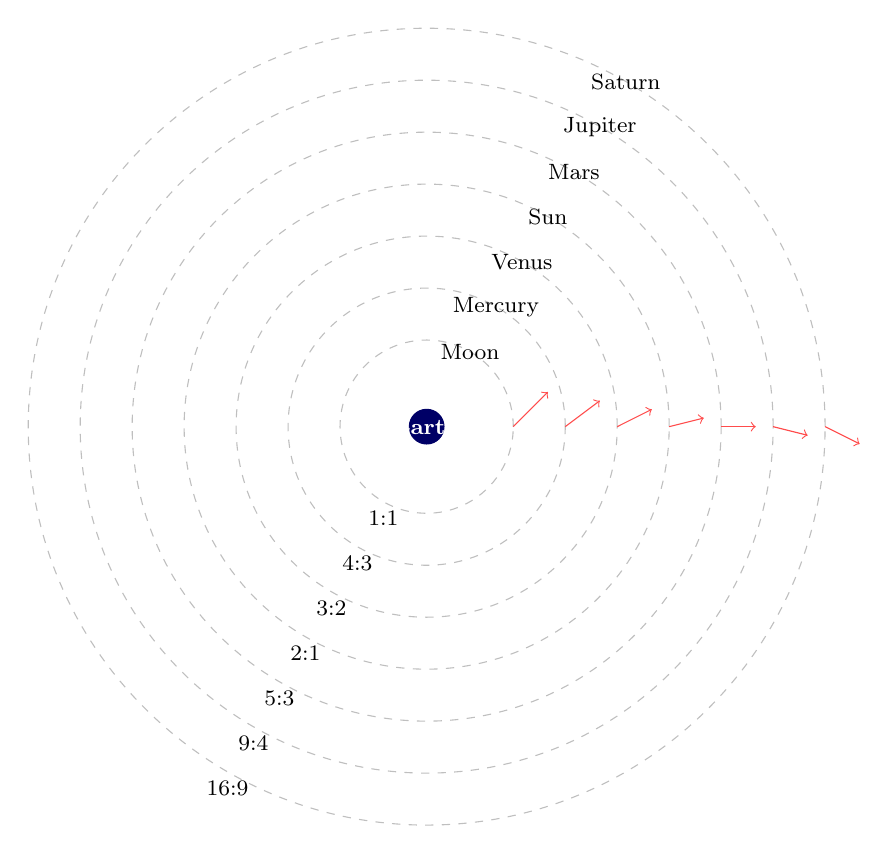
\begin{tikzpicture}[scale=2.2, every node/.style={font=\footnotesize}]
   
   % Central Earth
   \filldraw[blue!40!black] (0,0) circle (0.1) node[white] {\textbf{Earth}};
   
   % Radii, labels, and musical ratios
   \def\radii{{0.5, 0.8, 1.1, 1.4, 1.7, 2.0, 2.3}}
   \def\planets{{"Moon", "Mercury", "Venus", "Sun", "Mars", "Jupiter", "Saturn"}}
   \def\ratios{{"1:1", "4:3", "3:2", "2:1", "5:3", "9:4", "16:9"}}
   
   % Draw orbits and labels
   \foreach \r [count=\i] in {0.5, 0.8, 1.1, 1.4, 1.7, 2.0, 2.3} {
       \draw[gray!50, dashed] (0,0) circle (\r);
       \node at ({\r*cos(60)}, {\r*sin(60)}) {\pgfmathparse{\planets[\i-1]}\pgfmathresult};
       \node[below] at ({\r*cos(240)}, {\r*sin(240)}) {\pgfmathparse{\ratios[\i-1]}\pgfmathresult};
   }
   
   % Decorative arrows (hardcoded positions)
   \draw[->, red!70] (0.5, 0) -- ++(0.2, 0.2);
   \draw[->, red!70] (0.8, 0) -- ++(0.2, 0.15);
   \draw[->, red!70] (1.1, 0) -- ++(0.2, 0.1);
   \draw[->, red!70] (1.4, 0) -- ++(0.2, 0.05);
   \draw[->, red!70] (1.7, 0) -- ++(0.2, 0);
   \draw[->, red!70] (2.0, 0) -- ++(0.2, -0.05);
   \draw[->, red!70] (2.3, 0) -- ++(0.2, -0.1);
   
   \end{tikzpicture}
   \caption{The \textbf{Harmony of the Spheres}: In Pythagorean cosmology, planetary orbits were spaced according to musical ratios. The Moon and Mercury were closest to Earth and produced low tones; Saturn was farthest, producing the highest tone in this cosmic scale.}
\end{figure}

\medskip


Their obsession with ratios also led to a small crisis: the discovery of irrational numbers. Legend has it that when one of them proved that \(\sqrt{2}\) couldn’t be expressed as a ratio of whole numbers — shattering their belief that all things were number — he was either exiled or drowned at sea. Because nothing ruins a sacred worldview quite like math doing math.

In short, the Pythagoreans turned proportion into a metaphysical framework. Where Egyptians used ratios to survive floods, the Greeks used them to explain the cosmos, predict planetary motion, and — occasionally — justify throwing someone off a boat.
